\chapter{問題與討論}
\hspace{-1.7em} Q:gym用到的atari動態連結庫在讀取目錄下但在執行的時候出現缺少 ale\_ c.cp38-win\_ amd64.dll\\
\begin{figure}[hbt!]
\begin{center}
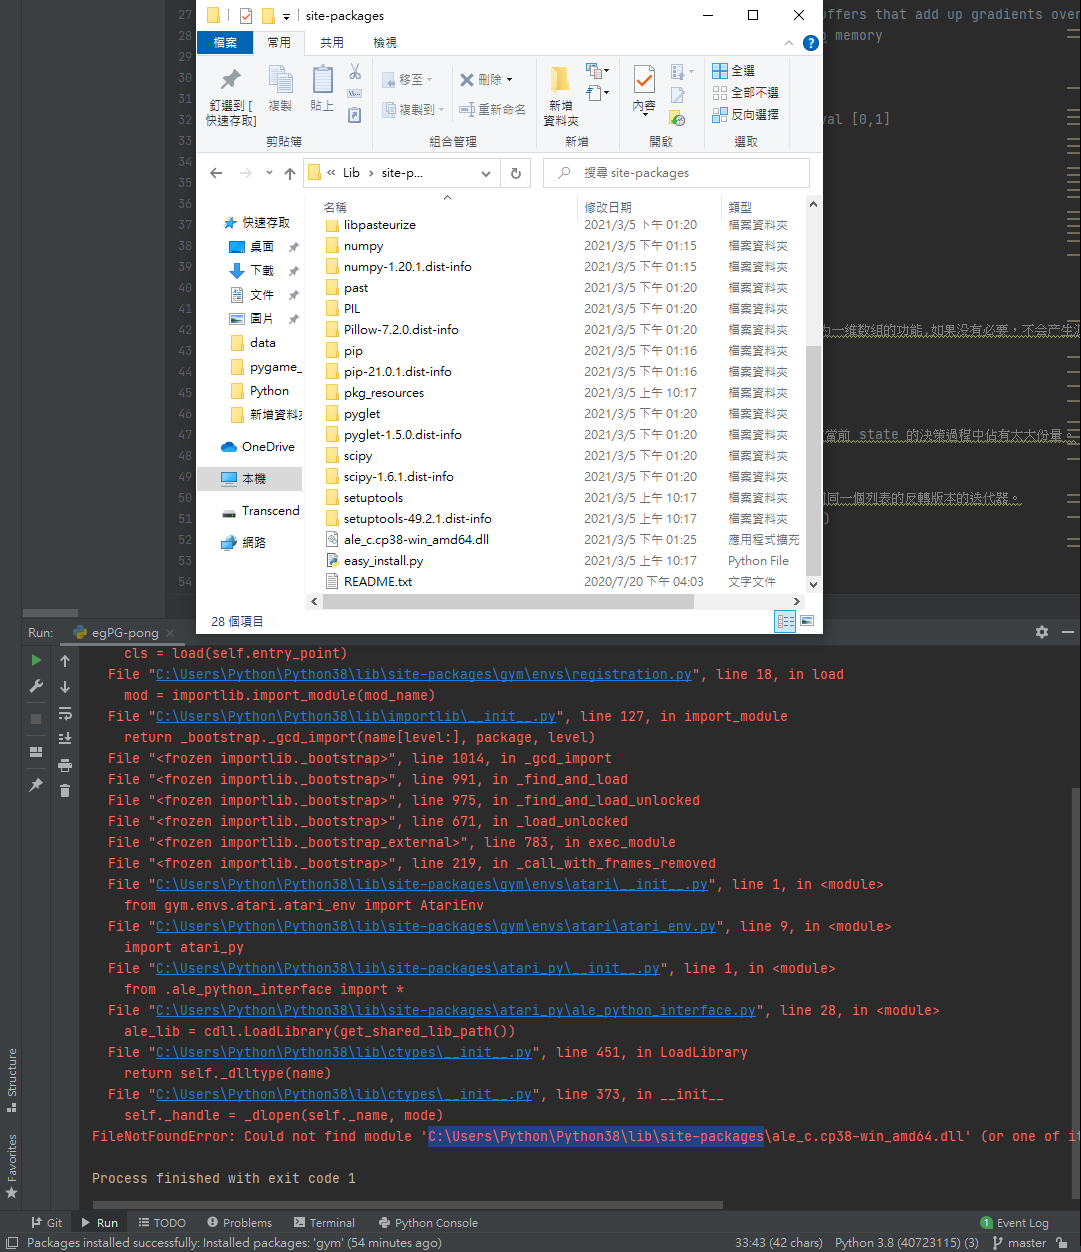
\includegraphics[width=15cm]{Q_dll}
\caption{\Large 動態連結庫錯誤}
\label{fig.動態連結庫錯誤}
\end{center}
\end{figure}
\newpage
\hspace{-1.4em}A:此問題尚未找到解決方法。\\
Q:錄製訓練過程的程式讀不到ffmpeg(圖.\ref{fig.Q_ffmpeg})。\\
\begin{figure}[hbt!]
\begin{center}
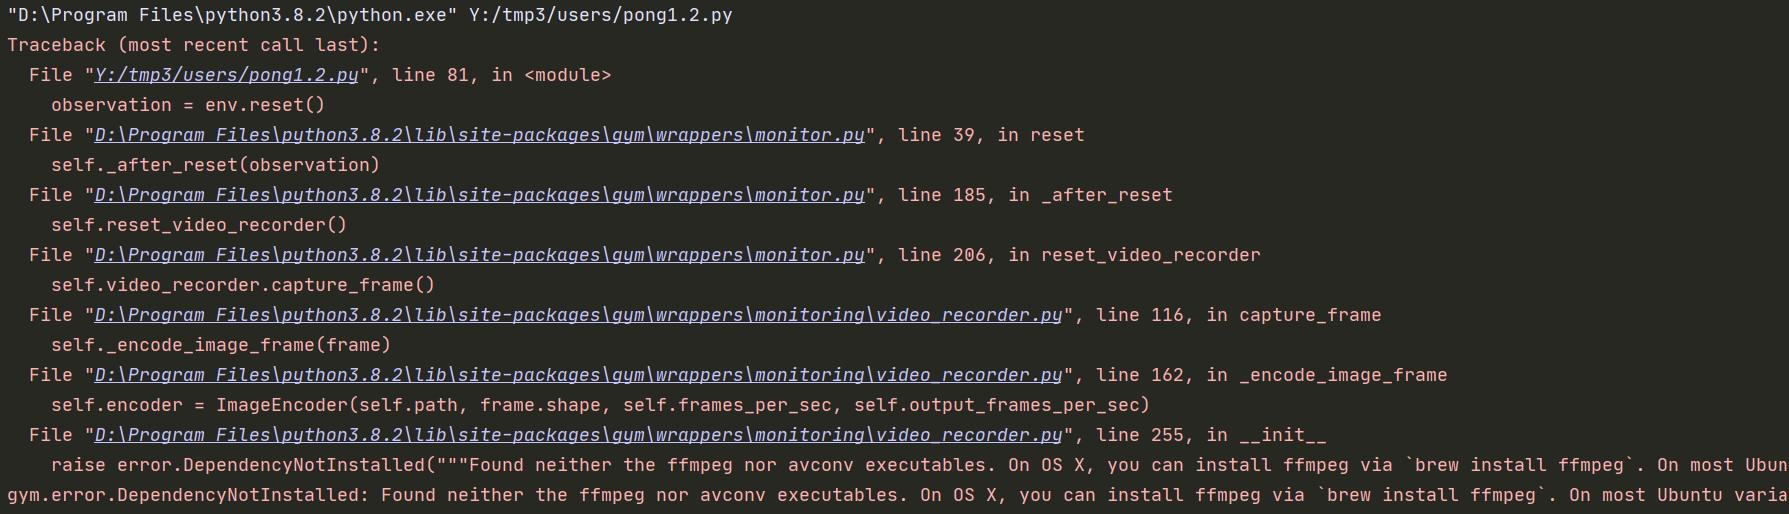
\includegraphics[width=15cm]{Q_ffmpeg}
\caption{\Large 程式讀不到ffmpeg}
\label{fig.Q_ffmpeg}
\end{center}
\end{figure}
\qquad \\
A:需要在作業系統中安裝ffmpeg:
\begin{enumerate}
\item 下載、解壓縮\\
先到官網 \href{https://ffmpeg.org/download.html}{https://ffmpeg.org/download.html} 下載" \href{https://www.gyan.dev/ffmpeg/builds/}{Windows builds from gyan.dev} ",下載 \href{https://www.gyan.dev/ffmpeg/builds/ffmpeg-git-full.7z}{https://www.gyan.dev/ffmpeg/builds/ffmpeg-git-full.7z} ,解壓縮重新命名成"ffmpeg"並放到C槽目錄下(C:$\setminus$ffmpeg)。
\item 環境設定(windows10 20H2 及 2004版本)\\
開啟"設定"→"系統"→左方"關於"選項→右側"進階系統設定"→"環境變數"(圖.\ref{fig.Q_ffmpeg-2})→選取"Path",編輯(圖.\ref{fig.Q_ffmpeg-3})→"新增",增加一個環境變數,給定內容為:"C:$\setminus$ffmpeg$\setminus$bin","確定"(圖.\ref{fig.Q_ffmpeg-4})→"確定"→"確定\\
\end{enumerate}
\begin{figure}[hbt!]
\begin{center}
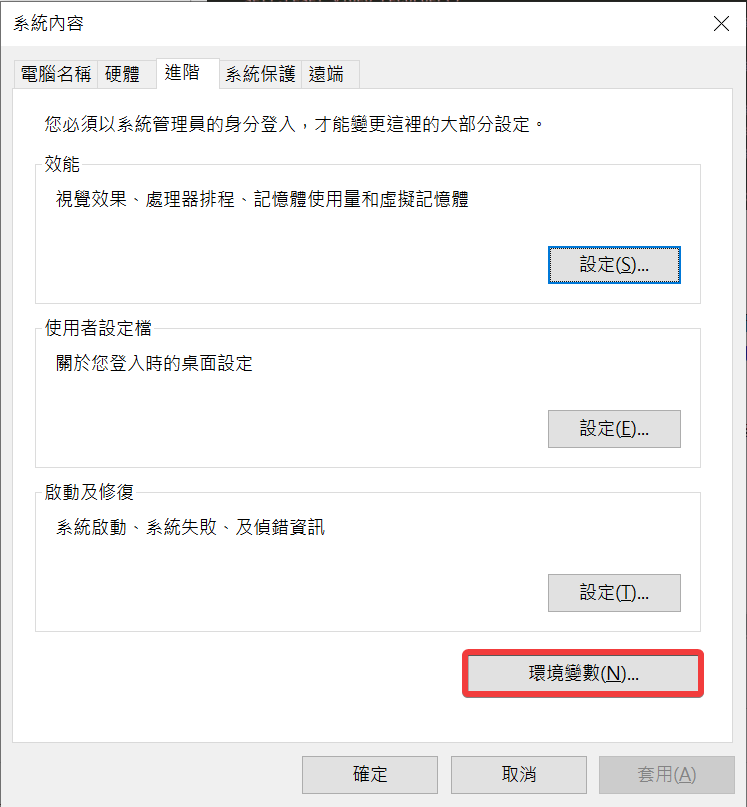
\includegraphics[width=10cm]{Q_ffmpeg-2}
\caption{\Large 進階系統設定}
\label{fig.Q_ffmpeg-2}
\end{center}
\end{figure}
\fontsize{0.001pt}{1pt}\selectfont .\\ %圖片間距勿刪
\begin{figure}[hbt!]
\begin{center}
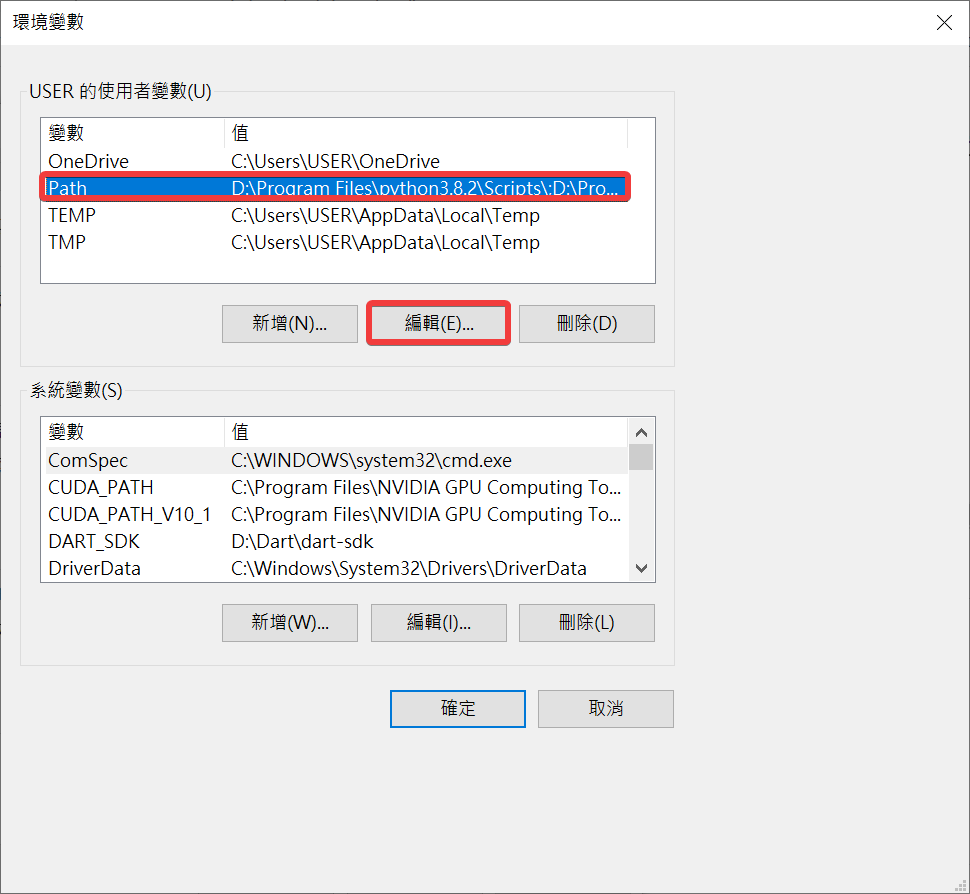
\includegraphics[width=10cm]{Q_ffmpeg-3}
\caption{\Large 環境變數}
\label{fig.Q_ffmpeg-3}
\end{center}
\end{figure}
\fontsize{0.001pt}{1pt}\selectfont .\\ %圖片間距勿刪
\newpage
\begin{figure}[hbt!]
\begin{center}
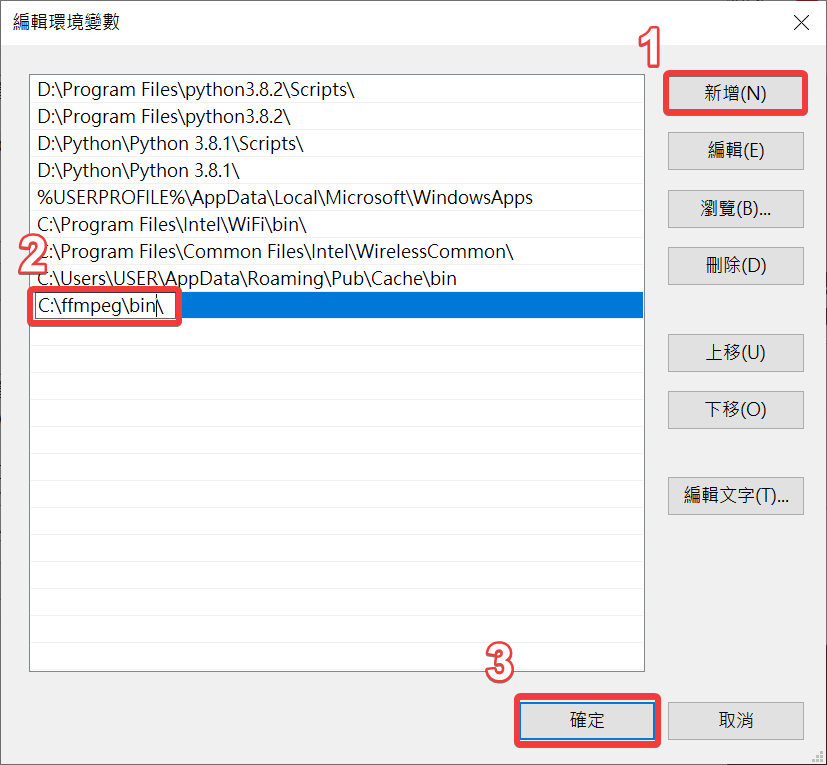
\includegraphics[width=15cm]{Q_ffmpeg-4}
\caption{\Large 編輯環境變數}
\label{fig.Q_ffmpeg-4}
\end{center}
\end{figure}
\fontsize{0.001pt}{1pt}\selectfont .\\ %圖片間距勿刪

\newpage %圖片間距勿刪
\fontsize{14pt}{28pt}\selectfont

\begin{itemize}
\item 測試\\
開啟命令字元(win+R,輸入"cmd"),執行"ffmpeg"(圖.\ref{fig.Q_ffmpeg-5})\\

\begin{figure}[hbt!]
\begin{center}
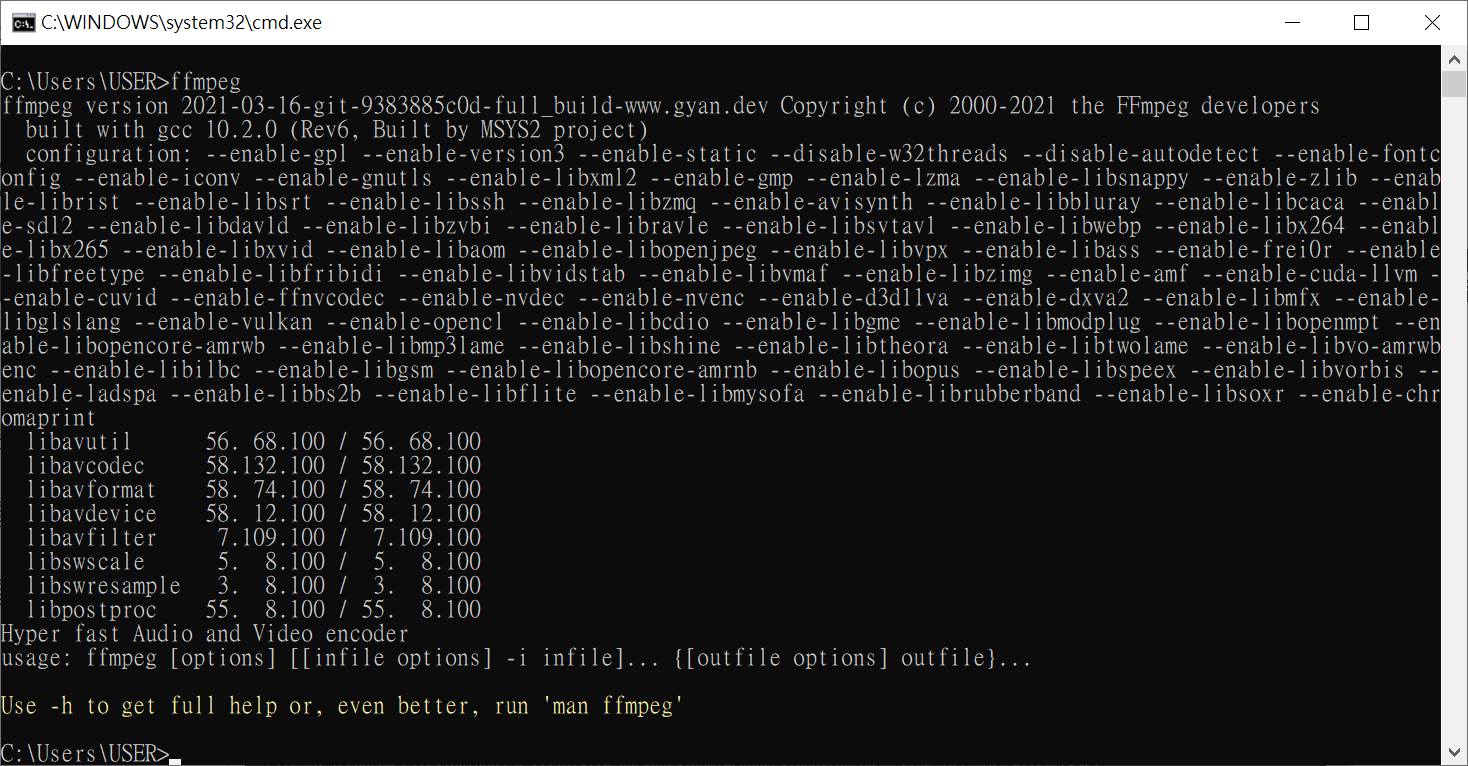
\includegraphics[width=15cm]{Q_ffmpeg-5}
\caption{\Large ffmpeg成功執行}
\label{fig.Q_ffmpeg-5}
\end{center}
\end{figure}
\end{itemize}
\newpage%圖片間距勿刪
\hspace{-1.7em} Q:運用gym.wrappers.Monitor透過ffmpeg進行錄影,紀錄下訓練影像。但記錄後的影像資料皆為1KB,並且無法開啟。(圖.\ref{fig.ffmpeg_mp4})\\
\begin{figure}[hbt!]
\begin{center}
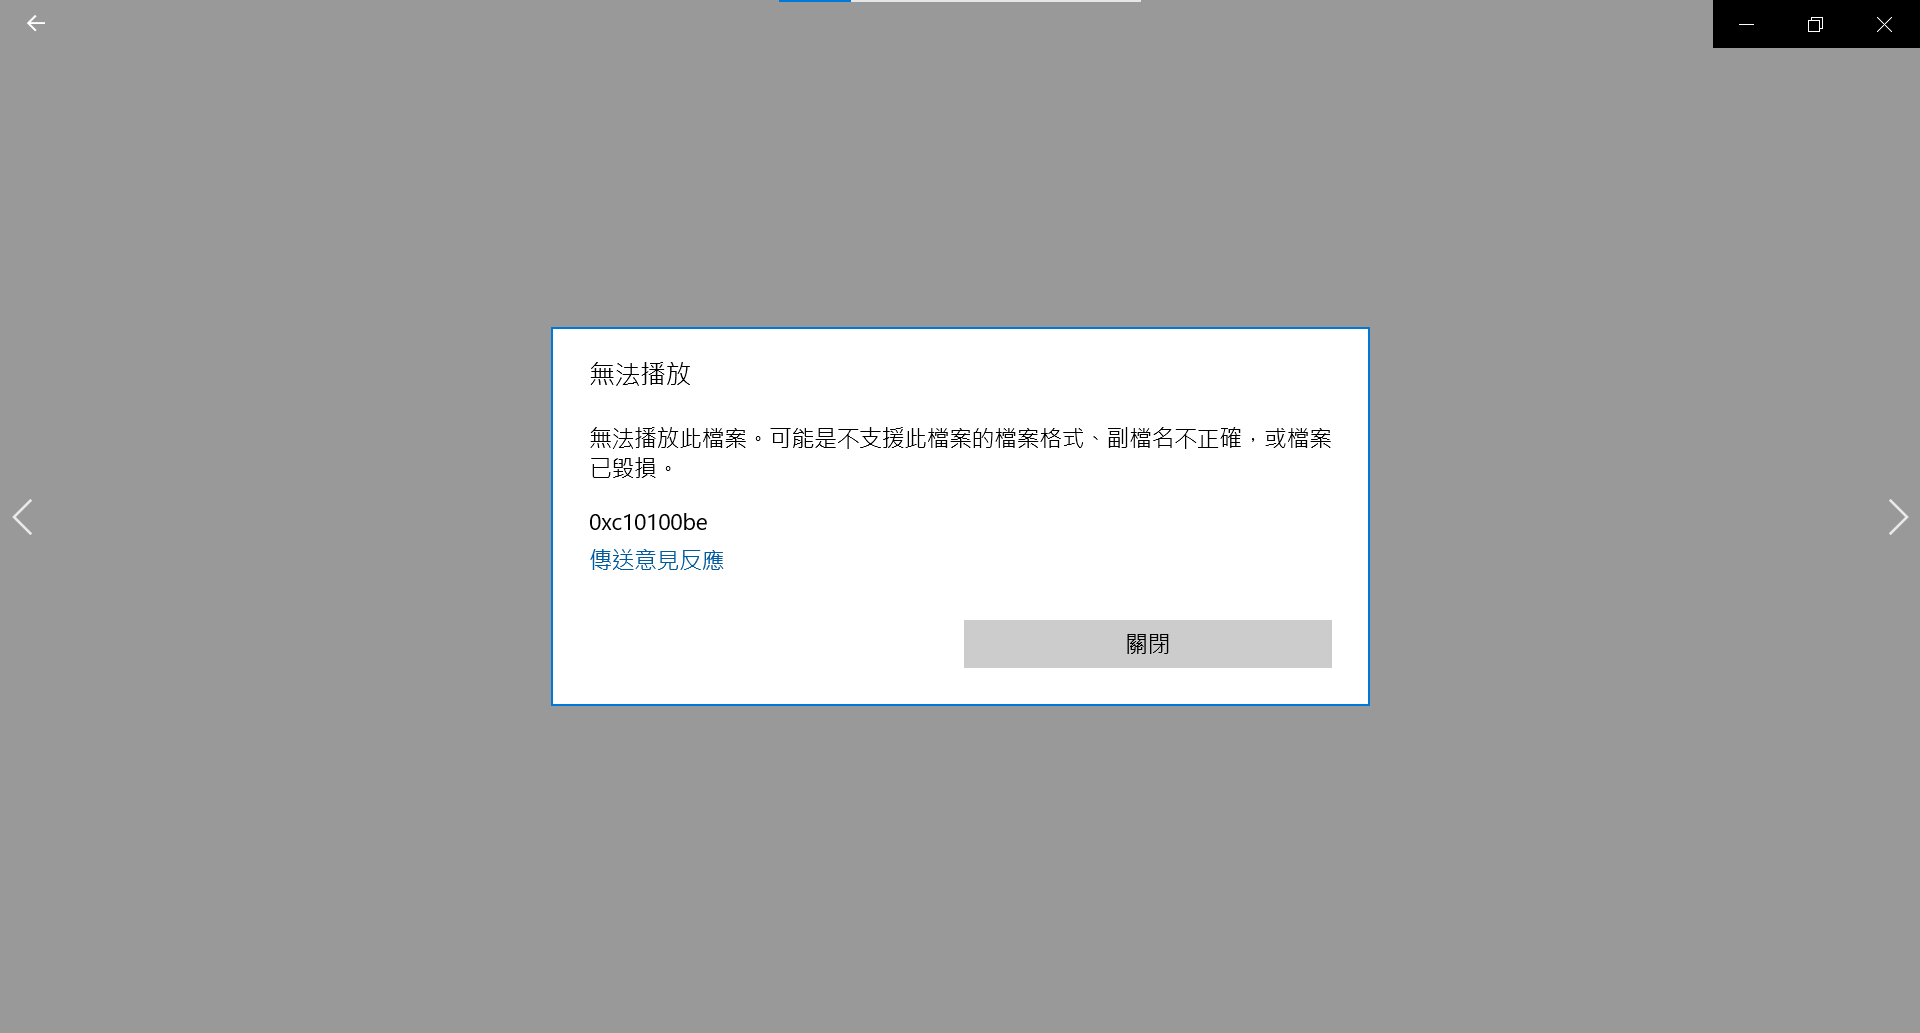
\includegraphics[width=15cm]{ffmpeg_mp4}
\caption{\Large 錄製後,影片無法開啟}
\label{fig.ffmpeg_mp4}
\end{center}
\end{figure}
\qquad \\%圖片間距勿刪
%圖片間距勿刪
A:修改g ym.wrappers.Monitor的video\_ recorder.py的設定(圖.\ref{fig.video_recorder}),將303行的縮排修正(從if階層上移到def的階層)即可(圖.)。\\
\begin{figure}[hbt!]
\begin{center}
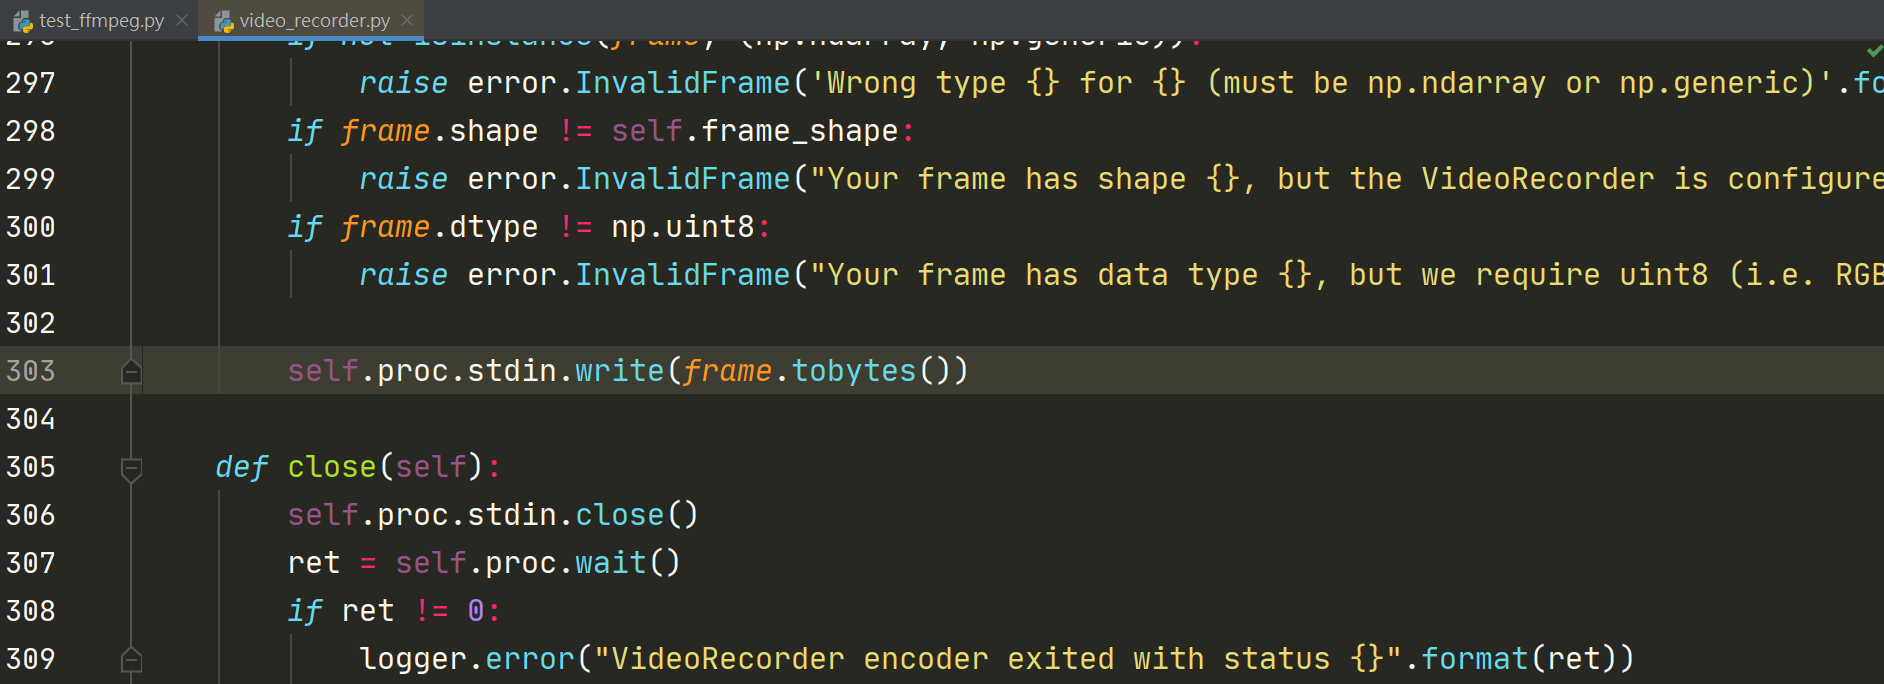
\includegraphics[width=15cm]{video_recorder}
\caption{\Large 原始設定}
\label{fig.video_recorder}
\end{center}
\end{figure}

\begin{figure}[hbt!]
\begin{center}
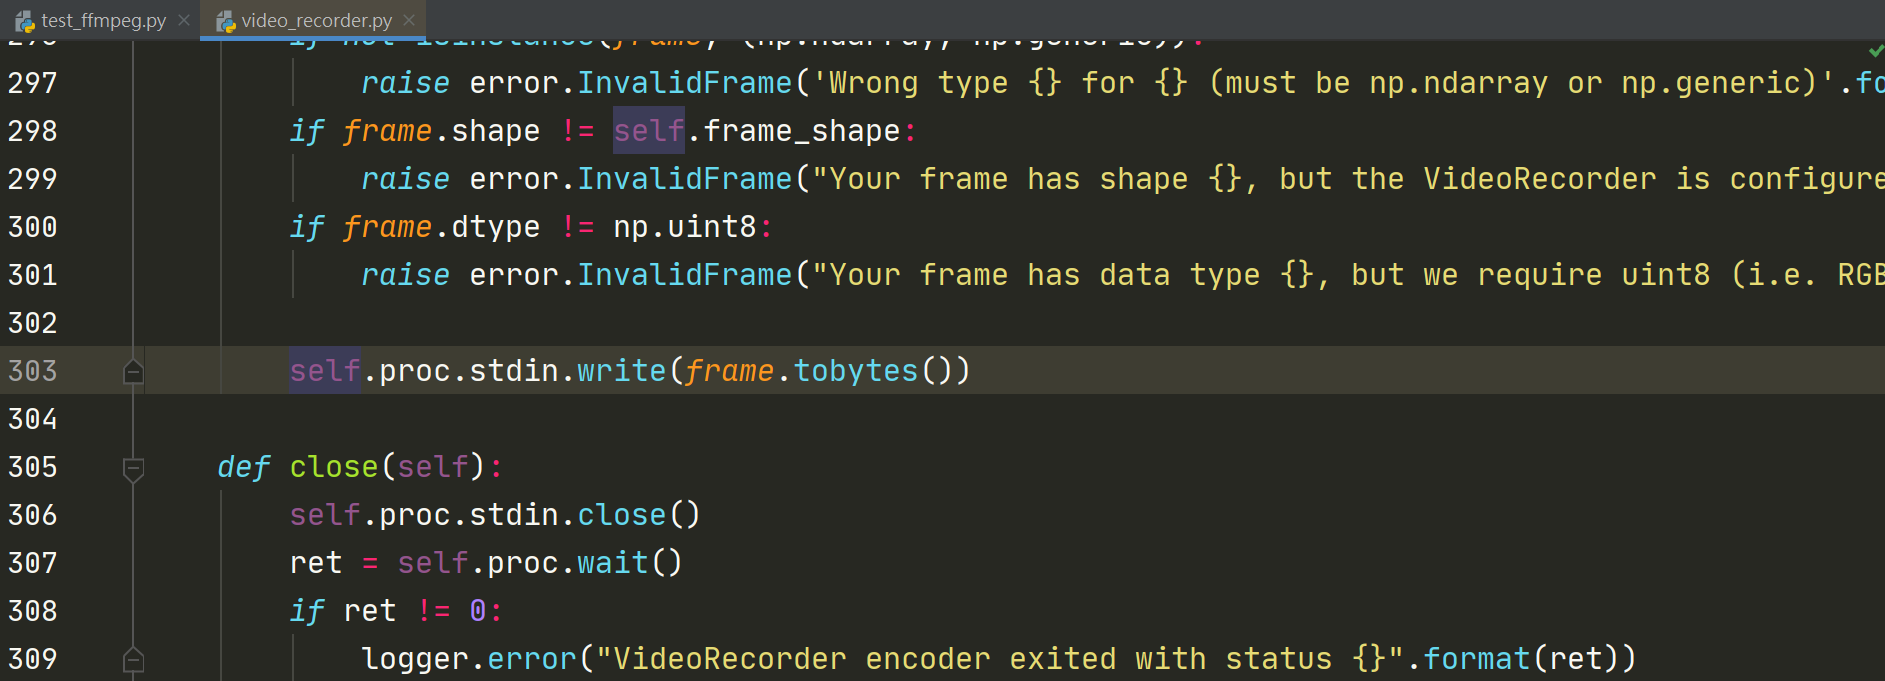
\includegraphics[width=15cm]{修正video_recorder}
\caption{\Large 修正後設定}
\label{fig.修正video_recorder}
\end{center}
\end{figure}
\newpage %圖片間距勿刪

\hspace{-1.7em} Q:啟用cmsimde的MathJax的功能遇到文章使用括號補充說明的內容被誤當成latex的語法轉換。\\
\hspace{-1.7em} A:格式轉換原始定義成"("和")",所以出現誤換的問題。\\
\begin{lstlisting}[caption=\Large\sectionef MathJax 程式碼]
<script>
  MathJax = {
    tex: {inlineMath: [['$', '$'], ['\\(', '\\)']]}
  };
  </script>
  <script id="MathJax-script" 
  async src="https://cdn.jsdelivr.net/npm/mathjax@3/es5/tex-chtml.js"> 
  </script>
\end{lstlisting}

修正後將"("和")"換成"\$",就解決誤換問題